% =====================================================================
% Multi-CNN Feature Fusion for HyperKvasir 23-class Classification
% Final report — SKELETON ONLY (Overleaf / pdfLaTeX compatible)
% Report language: Turkish (mandated by docs/report/AGENT_REPORT_RULES.md).
%
% RULES (see notes/report_notes.md):
%   - Do NOT invent results. Use \TODO{} where numbers/figures are not frozen.
%   - macro-F1 is the headline metric; accuracy is supporting only.
%   - Literature comparisons that use a different protocol are CONTEXTUAL only.
%   - No state-of-the-art claims.
% =====================================================================
\documentclass[11pt,a4paper]{article}

% --- Encoding & language (required for a Turkish report) ---------------
\usepackage[utf8]{inputenc}
\usepackage[T1]{fontenc}
\usepackage[turkish]{babel}

% --- Allowed common packages ------------------------------------------
\usepackage[margin=2.5cm]{geometry}
\usepackage{amsmath}
\usepackage{amssymb}   % \mathbb for fusion equations (Sec. Method)
\usepackage{graphicx}
\usepackage{booktabs}
\usepackage{tabularx}
\usepackage{float}
\usepackage{caption}
\usepackage{subcaption}
\usepackage{hyperref}   % keep last

\graphicspath{{figures/}}

% --- Simple TODO helper (visible in PDF, easy to grep) -----------------
\newcommand{\TODO}[1]{\textbf{\textcolor{red}{[TODO: #1]}}}
\usepackage{xcolor}

\hypersetup{
  colorlinks=true,
  linkcolor=black,
  citecolor=black,
  urlcolor=blue
}

% =====================================================================
\title{Çoklu CNN Tabanlı Özellik Füzyonu ile HiperKvasir\\
       23-Sınıf Gastrointestinal Görüntü Sınıflandırması}
\author{\TODO{Öğrenci 1 Ad Soyad, No} \and \TODO{Öğrenci 2 Ad Soyad, No}}
\date{\today}

\begin{document}

\maketitle

% ---------------------------------------------------------------------
% ABSTRACT — write LAST (per task rules). Keep as TODO until results frozen.
\begin{abstract}
\TODO{Özet en son yazılacak. Headline metrik macro-F1; accuracy destekleyici.
En iyi yapılandırma (üçlü weighted fine-tune, exp 11) ve resmi 5-fold protokol
vurgulanacak. Literatür karşılaştırmaları protokol farkı nedeniyle yalnızca
bağlamsaldır.}
\end{abstract}

% ---------------------------------------------------------------------
% =====================================================================
% 1. GİRİŞ (Introduction)
% Evidence base: project_plan.md §1, project_structure.md §2.4 (verified facts),
%                docs/school_assignment.md, docs/decisions.md,
%                docs/report/report_comparison_framework.md, references/INDEX.md.
% Rules: no results, no SOTA, macro-F1 headline, accuracy supporting only.
% =====================================================================
\section{Giriş}
\label{sec:introduction}

Bu projede ele alınan problem, gastrointestinal endoskopi görüntülerinin
HiperKvasir veri kümesindeki 23 sınıf üzerinde otomatik olarak
sınıflandırılmasıdır~\cite{borgli2020hyperkvasir}. Görevin temel zorluğu yalnızca
yüksek genel doğruluk elde etmek değil, sınıflar arasında oldukça dengesiz bir
dağılımın bulunduğu bir ortamda model davranışını anlamlı biçimde
değerlendirebilmektir. Bu nedenle çalışmada başarı ölçütü olarak tek başına
doğruluk (accuracy) değil, sınıf başına performansa duyarlı makro-F1 öne
çıkarılmıştır.

% --- Veri kümesinin zorluğu / dengesizlik ---
HiperKvasir etiketli alt kümesi 23 sınıf ve toplam 10.662 görüntü
içerir~\cite{borgli2020hyperkvasir}. Sınıf dağılımı ciddi biçimde dengesizdir:
en kalabalık sınıf (\textit{polyp}) yaklaşık 1028 örnek içerirken, en nadir
sınıf (\textit{hemorroids}) yalnızca 6 örnekle temsil edilmektedir.
Bu tür bir dağılımda, çoğunluk sınıflarında elde edilen yüksek doğruluk, nadir
sınıflardaki başarısızlığı gizleyebilir. Aggregate metrikler bu nedenle
yanıltıcı olabilir ve sınıf dengesizliğini açıkça dikkate alan bir değerlendirme
gerektirir.

% --- Çoklu CNN füzyonu motivasyonu ---
Farklı CNN mimarileri, aynı görüntüden farklı tümleyici temsiller öğrenme
eğilimindedir. Bu çalışmada üç önceden eğitilmiş omurga ağ --- ResNet50,
MobileNetV2 ve EfficientNetB0 --- özellik çıkarıcı olarak kullanılmış ve bu
ağlardan elde edilen özellik vektörleri birleştirilerek (özellik füzyonu) tek
bir temsil oluşturulmuştur. Buradaki temel soru, birden fazla omurga ağın
özelliklerini birleştirmenin tek bir omurga ağa kıyasla daha ayırt edici bir
temsil sağlayıp sağlamadığıdır. Gastrointestinal endoskopide çoklu-CNN özellik
füzyonu daha önce de incelenmiştir~\cite{ramamurthy2022effimix, ahmed2023hybrid};
ancak bu çalışmalar farklı protokoller kullandığından (Bölüm~\ref{sec:results})
yalnızca bağlamsal birer öncül olarak anılır, doğrudan karşılaştırma yapılmaz.

% --- Kontrollü karşılaştırma eksenleri ---
Çalışma, tek bir modelin performansını raporlamak yerine kontrollü
karşılaştırmalar üzerine kuruludur. Üç eksende karşılaştırma yapılır:
\begin{itemize}
  \item \textbf{Omurga ağ karşılaştırması:} ResNet50, MobileNetV2 ve
        EfficientNetB0'ın tek başına özellik çıkarıcı olarak performansı.
  \item \textbf{Füzyon karşılaştırması:} tek / ikili / üçlü omurga
        birleşimleri ile zorunlu iki füzyon yöntemi olan birleştirme
        (concatenation) ve ağırlıklı füzyonun (weighted fusion)
        karşılaştırılması; ek olarak gelişmiş bir kapılı füzyon (GMU) varyantı.
  \item \textbf{Transfer öğrenme karşılaştırması:} özelliklerin sabit tutulduğu
        (frozen) çıkarım ile son katman bloklarının ince ayarlandığı
        (fine-tuning) yaklaşımın karşılaştırılması.
\end{itemize}
Sınıflandırıcı tüm bu karşılaştırmalarda sabittir ve proje kararları gereği
yalnızca bir çok katmanlı algılayıcı (MLP) olarak seçilmiştir; bu nedenle
sınıflandırıcı bazlı bir karşılaştırma yapılmamıştır. Ödev metnindeki
``3 sınıflandırıcı'' ifadesinin sehven yazıldığı eğitmen tarafından teyit
edilmiştir; sınıflandırıcı MLP olarak sabitlenmiştir (PLD-06) ve karşılaştırmalar
yalnızca yukarıdaki üç eksende yapılır.

Bu üç temel eksene ek olarak, en iyi yapılandırmanın üzerinde toplamsal
(additive) ablasyonlar da değerlendirilmiştir: sınıf dengesizliğine duyarlı
focal loss, test zamanı veri artırma (TTA) ve sızıntısız seed topluluğu. Bu
ablasyonların hiçbiri, \%95 güven aralığı düzeyinde Week 3 çapraz-doğrulama
şampiyonunu (CE tabanlı en iyi yapılandırma) istatistiksel olarak geçememiştir;
final model olarak bu şampiyonun TTA'lı sürümü dondurulmuştur. Sayısal sonuçlar
ve dürüst değerlendirme Bölüm~\ref{sec:results} ve Bölüm~\ref{sec:discussion}'de
verilir.

% --- Metrik tercihi ve protokol ---
Değerlendirmede ana ölçüt olarak makro-F1 kullanılmış, doğruluk ise yalnızca
destekleyici bir ölçüt olarak raporlanmıştır. Makro-F1, her sınıfa eşit ağırlık
vererek nadir sınıflardaki başarısızlığı görünür kıldığı için dengesiz çok
sınıflı bir görevde daha bilgilendiricidir. Tüm karşılaştırmalar, sızıntıya
karşı denetlenmiş resmi HiperKvasir 5-katlı (5-fold) protokolü altında
yürütülmüş; böylece yapılandırmalar arasındaki karşılaştırmalar aynı bölme
mantığı üzerinde, metodolojik olarak tutarlı biçimde yapılmıştır.

% NOTE: Bu bölümün son paragrafı (projenin ana katkısına dair öğrencinin kendi
%       cümleleri) AGENT_REPORT_RULES.md §9 gereği öğrenci tarafından elle
%       gözden geçirilecektir.

% =====================================================================
% 2. YÖNTEM (Methodology)
% Evidence base: project_structure.md §2 (verified facts), configs/method/*.yaml,
%                configs/training/{frozen_extraction,finetune_wide}.yaml,
%                src/models/* docstrings, docs/decisions.md (PLD-04..08).
% Only IMPLEMENTED methods are described. No results here.
% =====================================================================
\section{Yöntem}
\label{sec:methodology}

Önerilen mimari üç bileşenden oluşur: önceden eğitilmiş CNN omurga ağları ile
özellik çıkarımı, bu özelliklerin ortak bir boyuta izdüşürülüp füzyonlanması ve
birleşik temsilin bir MLP sınıflandırıcı ile sınıflandırılması. Bu bölümde her
bileşen ve transfer öğrenme kurulumu açıklanmaktadır.

\begin{figure}[H]
\centering
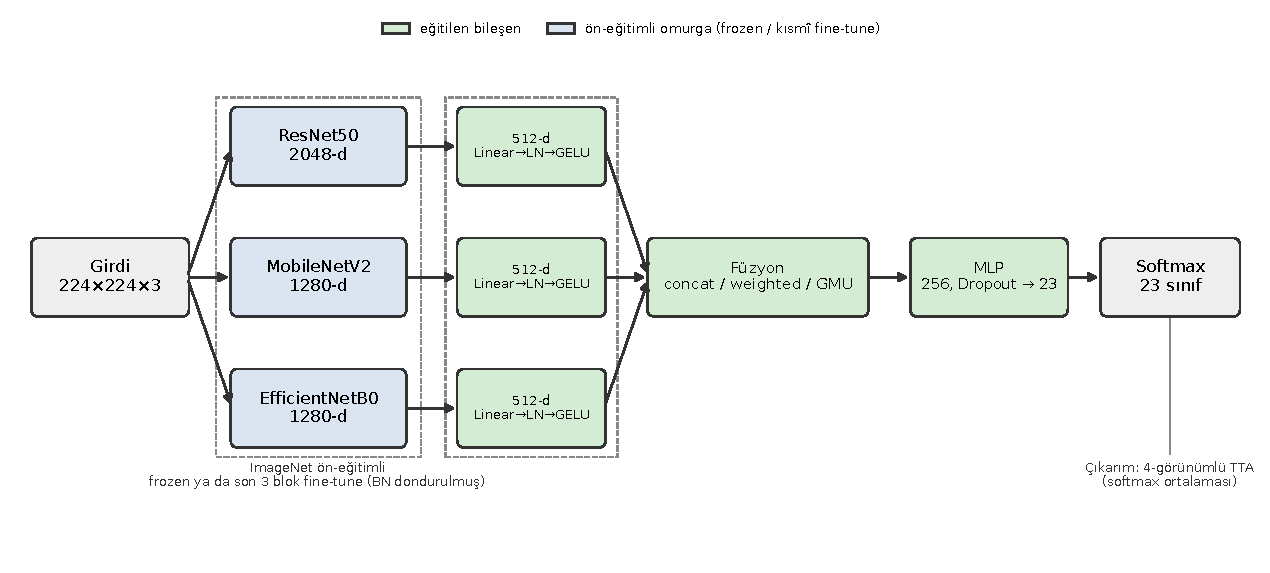
\includegraphics[width=\linewidth]{architecture.pdf}
\caption{Çoklu-CNN özellik füzyon mimarisi: üç önceden eğitilmiş omurga (ResNet50,
MobileNetV2, EfficientNetB0; frozen ya da son 3 blok fine-tune, BatchNorm
dondurulmuş) $\to$ 512-boyutlu dal projeksiyonu (Linear$\to$LayerNorm$\to$GELU)
$\to$ füzyon (concat / weighted / GMU) $\to$ MLP. Soldaki kesikli kutu omurgaları,
ortadaki kesikli kutu projeksiyon dallarını gösterir. Çıkarımda final model TTA
(base/hflip/scale/scale\_hflip; softmax ortalaması) kullanır.}
\label{fig:arch}
\end{figure}

\subsection{Omurga Ağlar (Özellik Çıkarıcılar)}
\label{subsec:backbones}
Üç omurga ağ olarak ResNet50~\cite{he2016resnet},
MobileNetV2~\cite{sandler2018mobilenetv2} ve
EfficientNetB0~\cite{tan2019efficientnet} kullanılır. Her ağ ImageNet üzerinde
önceden eğitilmiş torchvision uygulamasından alınır ve sınıflandırma başlığı
kaldırılarak son havuzlama (pooling) katmanından özellik vektörü elde edilir.
Çıkış özellik boyutları ResNet50 için 2048, MobileNetV2 ve EfficientNetB0 için
1280'dir.
Tüm görüntüler ağlara $224\times224$ çözünürlükte ve ImageNet ortalama/standart
sapma değerleriyle normalize edilerek verilir; böylece üç omurga ağ kontrollü
ve karşılaştırılabilir koşullarda çalışır.

\subsection{Projeksiyon Katmanı}
\label{subsec:projection}
Omurga ağların özellik boyutları birbirinden farklı olduğundan (2048'e karşı
1280), füzyondan önce her dal ortak bir boyuta izdüşürülür. Her omurga ağın
özelliği 512 boyutlu bir projeksiyona eşlenir; bu projeksiyon kavramsal olarak
bir doğrusal katman, ardından katman normalizasyonu (LayerNorm) ve GELU
aktivasyonundan oluşur. Bu adım hem boyut uyumsuzluğunu giderir
hem de farklı ölçeklerdeki özellikleri füzyon için ortak bir temsile getirir.

\subsection{Birleştirme (Concatenation) Füzyonu}
\label{subsec:concat}
Birleştirme füzyonu, projeksiyon sonrası dal özelliklerini özellik ekseninde
uç uca ekleyerek tek bir vektör oluşturur. $N$ dal için her biri 512 boyutlu
olduğundan birleşik temsil $N\times512$ boyutludur (ör. üçlü birleşimde 1536).
Bu yöntem öğrenilebilir bir füzyon parametresi içermez ve tüm dalların bilgisini
eşit biçimde aşağı akışa taşır.

\subsection{Ağırlıklı (Weighted) Füzyon}
\label{subsec:weighted}
Ağırlıklı füzyon, dalların katkısını öğrenilebilir kılar. $N$ dal için
$\mathbf{a}\in\mathbb{R}^{N}$ öğrenilebilir bir parametre vektörüdür (uygulamada
sıfırlarla, yani düzgün başlangıçla ilklendirilir). Dal ağırlıkları bu vektörün
softmax'ı ile elde edilir ve projekte edilmiş dal özelliklerinin
$\mathbf{x}_i\in\mathbb{R}^{512}$ ağırlıklı toplamı alınır:
\begin{equation}
  \mathbf{w} = \operatorname{softmax}(\mathbf{a}), \qquad
  \mathbf{h} = \sum_{i=1}^{N} w_i\,\mathbf{x}_i ,
\end{equation}
burada $\sum_i w_i = 1$ ve birleşik temsil $\mathbf{h}$ yine 512 boyutludur.
Birleştirme füzyonundan farkı, hangi omurga ağın temsiline ne ölçüde
güvenileceğinin eğitim sırasında ayarlanabilmesidir.

\subsection{Gelişmiş Füzyon: GMU (İsteğe Bağlı Eksen)}
\label{subsec:gmu}
Zorunlu iki füzyon yöntemine ek olarak, gelişmiş bir kapılı çok-kipli birim
(Gated Multimodal Unit, GMU) varyantı da uygulanmış ve aynı protokol altında
değerlendirilmiştir~\cite{arevalo2017gmu}. Sabit ağırlıklı füzyondan farklı
olarak GMU, kapı (gate) ağırlıklarını her örnek için ayrı hesaplar. Bu projede
Arevalo ve ark.\ §3.1'deki iki-kipli formülasyonun $N$-dal softmax
genelleştirmesi kullanılır:
\begin{align}
  \mathbf{h}_i &= \tanh(W_i\,\mathbf{x}_i), \qquad i = 1,\dots,N \\
  \mathbf{z}   &= \operatorname{softmax}\!\big(W_z\,[\mathbf{x}_1,\dots,\mathbf{x}_N]\big) \in \mathbb{R}^{N} \\
  \mathbf{h}   &= \sum_{i=1}^{N} z_i\,\mathbf{h}_i ,
\end{align}
burada $[\cdot,\dots,\cdot]$ birleştirme işlemidir ve $W_z$ kapısı, dönüşümden
önceki ham dal özelliklerini girdi olarak alır (paper §3.1). Softmax, iki-kipli
$\sigma/(1-\sigma)$ çiftini, ağırlıkları toplamı 1 olan $N$-yönlü bir yarışmaya
genelleştirir.

\subsection{MLP Sınıflandırıcı}
\label{subsec:mlp}
Birleşik özellik vektörü, tek bir çok katmanlı algılayıcı (MLP) ile 23 sınıfa
sınıflandırılır. Sınıflandırıcı bir gizli katman (boyut 256) ve 0,3 oranında
dropout içerir. Sınıflandırıcı tüm deneylerde MLP olarak sabit tutulmuştur;
SVM, RandomForest veya XGBoost gibi alternatif sınıflandırıcılar
değerlendirilmemiştir. Bu sayede karşılaştırmalar omurga ağ,
füzyon ve transfer öğrenme eksenlerinde yoğunlaşır.

\subsection{Frozen Çıkarım ve Fine-tuning}
\label{subsec:transfer}
İki transfer öğrenme yaklaşımı karşılaştırılır:
\begin{itemize}
  \item \textbf{Frozen özellik çıkarımı:} Omurga ağların ağırlıkları
        dondurulur; özellikler bir kez çıkarılıp önbelleğe alınır ve yalnızca
        projeksiyon, füzyon ve MLP bileşenleri eğitilir.
  \item \textbf{Fine-tuning:} Her omurga ağın son üç bloğu çözülerek uçtan uca
        eğitilir. Bu kurulumda katman bazlı azalan öğrenme oranı (LLRD)
        kullanılır ve dondurulmuş bloklardaki BatchNorm istatistikleri,
        proje kuralı gereği güncellenmeden tutulur.
\end{itemize}
Her iki yaklaşımda da sınıf dengesizliği eğitim aşamasında ağırlıklı örnekleme
(weighted sampler) ile ele alınır. Eğitim ayrıntıları ve hiperparametreler
Bölüm~\ref{sec:setup}'te verilmiştir.

\subsection{Sınıf Dengesizliğine Duyarlı Kayıp: Focal Loss (Ablasyon)}
\label{subsec:focal}
Sınıf dengesizliğini kayıp düzeyinde ele almak için en iyi yapılandırma (exp 11,
üçlü ağırlıklı fine-tune) üzerinde tek değişkenli bir ablasyon olarak focal
loss~\cite{lin2017focal} denenmiştir. Lin ve ark.\ §3.2, eşitlik
(5)'teki $\alpha$-dengeli biçim kullanılır:
\begin{equation}
  \mathrm{FL}(p_t) = -\,\alpha_t\,(1 - p_t)^{\gamma}\,\log(p_t),
\end{equation}
burada $p_t$ gerçek sınıfın model olasılığı, $\gamma \ge 0$ odaklama
parametresidir; paper'ın önerdiği $\gamma = 2{,}0$ alınmıştır. $(1-p_t)^{\gamma}$
modülasyon çarpanı kolay örnekleri ($p_t > 0{,}5$) baskılayıp eğitimi zor
örneklere yöneltir. Bu ablasyon, focal loss ile etiket yumuşatmayı kasıtlı
olarak \emph{birleştirmez}: etiket yumuşatma hedef dağılımını değiştirir ve
$p_t$'ye dayanan focal modülasyonuyla çakışır. Bu nedenle focal yapılandırması,
exp 11'in CE yapılandırmasından yalnızca kayıp bloğunda ayrılır; diğer tüm
hiperparametreler aynıdır (temiz, tek değişkenli karşılaştırma).

\subsection{Test Zamanı Veri Artırma (TTA)}
\label{subsec:tta}
Nihai modelin çıkarım reçetesi, eğitim maliyeti olmadan uygulanan
deterministik bir test zamanı veri artırmadır (TTA). Her görüntü için dört
deterministik görünüm üretilir --- (i) \emph{base}: Resize(256)$\rightarrow$
CenterCrop(224); (ii) \emph{hflip}: base + yatay çevirme; (iii) \emph{scale}:
Resize(224)$\rightarrow$CenterCrop(224); (iv) \emph{scale\_hflip}: scale + yatay
çevirme --- ve bu görünümlerin softmax olasılıkları görüntü başına ortalanır. TTA
\emph{model başına} ve \emph{örnek başına} uygulanır; herhangi bir kat (fold)
sınırını aşmadığından sızıntıya yol açmaz.

\subsection{Sızıntısız Seed Topluluğu (Ensemble)}
\label{subsec:ensemble}
Resmi 5-katlı protokolde yalnızca sızıntısız topluluk yöntemine izin verilir.
Seed topluluğu, aynı yapılandırmanın farklı tohumlarla (seed)
eğitilmiş modellerinin softmax olasılıklarını \emph{her katın kendi ayrık test
kümesi içinde} ortalayıp ardından 5 katı havuzlayarak her örneğin tam olarak bir
kez görünmesini sağlar ($n = 10{.}662$). Olasılıklar her zaman softmax düzeyinde
ortalanır; argmax oylaması kullanılmaz. Katlar arası saf model ortalaması bu
çalışmada kullanılmamıştır: 5 kat modelini tüm veri kümesi üzerinde ortalamak
sızıntıya yol açar,
çünkü her örnek katların 4'ünün eğitim kümesinde yer almıştır. Bu nedenle
modeller hiçbir zaman katlar arasında topluluk haline getirilmez.

% =====================================================================
% 3. DENEYSEL KURULUM (Experimental Setup)
% Evidence base: configs/dataset/hyperkvasir_23class_official.yaml,
%                configs/training/finetune_wide.yaml, docs/decisions.md
%                (2026-05-23 split protocol, D-09 provenance), docs/environment.md,
%                docs/results_progress.md, src/evaluation/{metrics,statistical}.py.
% Only documented values. No fabricated hardware/runtime.
% =====================================================================
\section{Deneysel Kurulum}
\label{sec:setup}

\subsection{Veri Kümesi}
\label{subsec:dataset}
Deneyler HiperKvasir etiketli alt kümesi üzerinde yürütülür: 23 sınıf, toplam
10.662 JPEG görüntü, CC BY 4.0 lisansı~\cite{borgli2020hyperkvasir}. Sınıf
dağılımı dengesizdir ve bu durum değerlendirme metriklerinin seçimini doğrudan
etkilemektedir (bkz. Bölüm~\ref{subsec:metrics}). Tüm görüntüler ön işleme
aşamasında kısa kenarı 256'ya ölçeklenip $224\times224$ boyutuna kırpılır ve
ImageNet ortalama/standart sapma değerleriyle normalize edilir.

\subsection{Değerlendirme Protokolü}
\label{subsec:protocol}
Birincil değerlendirme protokolü resmi HiperKvasir 5-katlı (5-fold) bölmesidir
(karar tarihi 2026-05-23). Manifestler resmi katlardan deterministik olarak
türetilir: $k$ katı için resmi kat $k$ test, kat $(k+1)\bmod 5$ doğrulama
(validation) ve kalan katlar eğitim olarak kullanılır. Bölme manifestleri
kaydedilir ve eğitim/doğrulama/test bölümleri arasında veri sızıntısına karşı
denetlenir. Bu protokol, yapılandırmalar arasındaki tüm iç
karşılaştırmaların aynı bölme mantığı üzerinde yapılmasını sağlar.

\subsection{Metrikler}
\label{subsec:metrics}
Ana başarı ölçütü makro-F1'dir. Buna ek olarak doğruluk (accuracy),
makro kesinlik (macro precision) ve makro duyarlılık (macro recall) destekleyici
ölçütler olarak raporlanır. Sınıf dengesizliğinin etkisini görünür kılmak için
mikro-F1 (tek etiketli çok sınıflı durumda doğruluğa eşittir), örnek-ağırlıklı
(weighted) F1 ve Matthews korelasyon katsayısı (MCC) de ek ölçütler olarak
hesaplanmıştır. Makro-F1'in öne çıkarılmasının nedeni, her sınıfa eşit ağırlık
vererek nadir sınıflardaki başarısızlığı görünür kılması ve bu sayede dengesiz
bir veri kümesinde aggregate doğruluğun yaratabileceği iyimser yanılgıyı
önlemesidir; makro-F1 ile örnek-ağırlıklı F1 arasındaki belirgin fark, bu
dengesizliğin doğrudan kanıtıdır. Tüm metrikler sıfır-bölme durumlarına karşı
güvenli biçimde hesaplanır.

Sınıf düzeyindeki davranışı incelemek için en iyi model için sınıf başına
kesinlik/duyarlılık/F1 ve destek (support) değerleri (Tablo~\ref{tab:perclass})
ile bir hata
matrisi (confusion matrix) sunulur; sayısal değerler ve referanslar
Bölüm~\ref{sec:results}'te verilir.
Değerlendirmenin güvenilirliğini güçlendirmek için seçilmiş yapılandırmalarda
5-kat ortalaması $\pm$ standart sapma raporlanır; ayrıca \%95 güven aralıkları
önyükleme (bootstrap) ile hesaplanır. Güven aralığı yöntemi yüzdelik
(percentile) tabanlıdır: 5 katın görüntü-başı tahminleri havuzlanır
($n = 10{.}662$, her örnek tam bir kez) ve bu havuz üzerinde $1000$ önyükleme
örneklemesi (sabit tohum 42) ile hesaplanır. Sayısal değerler
Bölüm~\ref{sec:results}'te verilir.

\subsection{Hiperparametreler}
\label{subsec:hyperparams}
İnce ayar deneyleri ortak bir ince-ayar yapılandırması kullanır.
Eniyileyici AdamW'dir~\cite{loshchilov2019adamw} (başlık öğrenme oranı
$1\times10^{-3}$, omurga öğrenme oranı $1\times10^{-4}$, ağırlık sönümü
$1\times10^{-4}$); fine-tuning sırasında katman bazlı azalan öğrenme oranı
(LLRD, sönüm katsayısı 0,75) uygulanır. Öğrenme oranı programı, 5 epoch ısınmalı
(warmup) kosinüs tavlamasıdır. Kayıp fonksiyonu, 0,1 etiket yumuşatmalı (label
smoothing) çapraz entropidir. Veri artırma olarak RandAugment ($N{=}2$, $M{=}9$),
CutMix~\cite{yun2019cutmix} ($\alpha{=}1{,}0$, olasılık 0,5) ve yatay çevirme
kullanılır. Ağırlıkların üstel hareketli ortalaması (EMA, sönüm 0,999, 5.\
epoch'tan itibaren) tutulur. Eğitim en fazla 60 epoch sürer; doğrulama
makro-F1'i üzerinde 8 epoch sabırlı erken durdurma uygulanır ve toplu iş boyutu
(batch size) 64'tür. Sınıf dengesizliği eğitimde ağırlıklı örnekleme ile ele
alınır. Frozen deneyler aynı temel kurulumu kullanır; ancak omurga ağ blokları
çözülmez ve önbelleğe alınmış özellikler üzerinde yalnızca başlık eğitilir.

Focal loss ablasyonu (Bölüm~\ref{subsec:focal}) temel yapılandırmadan yalnızca
kayıp bloğunda ayrılır (etiket yumuşatmalı CE yerine $\gamma{=}2{,}0$ focal;
etiket yumuşatma kaldırılmıştır). Nihai modelin değerlendirilmesinde,
Bölüm~\ref{subsec:tta}'da tanımlanan dört-görünümlü deterministik TTA çıkarımı
kullanılır.

\subsection{Yeniden Üretilebilirlik ve Ortam}
\label{subsec:repro}
Belirlenebilirlik (determinism) için raporlanan koşularda sabit tohum (seed 42)
ve deterministik mod kullanılmıştır. Yerel ortam şudur: Python 3.11.9, PyTorch
2.12.0+cu132, torchvision 0.27.0+cu132 ve NVIDIA GeForce RTX 5080 dizüstü GPU'su.
Raporlanan 5-katlı çapraz doğrulama ve nihai model bu yerel ortamda üretilmiştir;
daha hızlı keşif için isteğe bağlı bir Colab A100 yolu da aynı bilimsel ayarlarla
kullanılabilmektedir. Tüm koşular için yapılandırma, metrik çıktıları ve epoch
günlükleri proje dosyaları içinde saklanır; böylece rapordaki her sayı
izlenebilir.

% =====================================================================
% 4. SONUÇLAR (Results)
% Use ONLY documented numbers (traceable to results/tables/, results/figures/,
% docs/FINAL_MODEL.md). No invention. macro-F1 headline; accuracy supporting.
% Sources:
%   Table 1  -> results/tables/ablation_table.md (fold-0 rows)
%   Table 2  -> results/tables/cv_*_summary.json
%   Table 2b -> results/tables/ci_*.json
%   Supporting metrics -> results/tables/extra_metrics_*.json
%   Table 3  -> results/tables/per_class_frozen_tta.md
%   Table 4  -> results/tables/training_time.md
%   Week 3.5 head-to-head -> ci_11_*{,_tta,_ensemble,_ensemble_tta}.json, ci_16_*
%   Figures  -> results/figures/{comparison_bar_chart,training_curves,
%               confusion_matrix_frozen_tta,per_class_f1_frozen_tta}.png
% =====================================================================
\section{Sonuçlar}
\label{sec:results}

Sonuçlar dört eksende sunulur: (i) fold-0 üzerinde tek/ikili/üçlü ablasyon,
(ii) seçilmiş yapılandırmalar için 5-katlı çapraz doğrulama (CV), (iii) en iyi
yapılandırma üzerinde toplamsal ablasyonların baş-başa
karşılaştırması ve (iv) nihai modelin sınıf-bazlı çözümlemesi. Ana ölçüt
makro-F1, destekleyici ölçüt ise doğruluktur (accuracy).

\subsection{Tek/İkili/Üçlü Ablasyon (fold-0)}
\label{subsec:t1}
Tablo~\ref{tab:ablation} fold-0 üzerindeki ablasyonu özetler. Frozen rejimde en
iyi tekil omurga EfficientNetB0 (makro-F1 $0{,}5586$), en iyi yapılandırma ise
M+E birleştirme çiftidir ($0{,}5758$); ResNet50'nin frozen üçlü birleştirmeye
eklenmesi makro-F1'i düşürür. Fine-tune rejiminde fold-0'da en yüksek değeri
üçlü birleştirme verir ($0{,}5796$); ancak bu sıralamanın CV ile tersine döndüğü
Bölüm~\ref{subsec:t2}'de görülecektir. Hiçbir koşuda NaN değer veya sıfır-destekli
sınıf oluşmamıştır.

\begin{table}[H]
\centering
\caption{Fold-0 ablasyonu (resmi 5-katlı bölme, fold 0). Acc = doğruluk,
M-F1 = makro-F1.}
\label{tab:ablation}
\begin{tabular}{llll cc}
\toprule
ID & Omurga(lar) & Füzyon & Rejim & Acc & M-F1 \\
\midrule
01 & ResNet50        & --       & frozen        & 0.8402 & 0.5588 \\
02 & MobileNetV2     & --       & frozen        & 0.8483 & 0.5502 \\
03 & EfficientNetB0  & --       & frozen        & 0.8591 & 0.5586 \\
05 & R+M             & concat   & frozen        & 0.8247 & 0.5438 \\
06 & R+E             & concat   & frozen        & 0.8388 & 0.5464 \\
07 & M+E             & concat   & frozen        & 0.8728 & \textbf{0.5758} \\
08 & R+M+E           & concat   & frozen        & 0.8567 & 0.5630 \\
09 & R+M+E           & weighted & frozen        & 0.8549 & 0.5609 \\
\midrule
12 & ResNet50        & --       & finetune-3blk & 0.8501 & 0.5748 \\
13 & EfficientNetB0  & --       & finetune-3blk & 0.8355 & 0.5539 \\
14 & M+E             & concat   & finetune-3blk & 0.8384 & 0.5522 \\
10 & R+M+E           & concat   & finetune-3blk & 0.8784 & \textbf{0.5796} \\
11 & R+M+E           & weighted & finetune-3blk & 0.8685 & 0.5751 \\
15 & R+M+E           & GMU      & finetune-3blk & 0.8497 & 0.5645 \\
\bottomrule
\end{tabular}
\end{table}

\subsection{Seçilmiş 5-Katlı Çapraz Doğrulama}
\label{subsec:t2}
Seçilmiş beş yapılandırma beş katın tamamında çalıştırılmıştır
(Tablo~\ref{tab:cv}). En iyi CV yapılandırması üçlü ağırlıklı fine-tune'dur
(exp 11, makro-F1 $0{,}5892 \pm 0{,}0102$). Bu, fold-0'da birleştirmenin
($0{,}5796$) ağırlıklıyı ($0{,}5751$) geçtiği sıralamayı tersine çevirir;
fold-0 bu iki yapılandırma için temsil edici olmayan bir örnektir. GMU, CV
düzeyinde birleştirmeyi geçmez (fark $\approx 0{,}002$, gürültü içinde).

\begin{table}[H]
\centering
\caption{Seçilmiş 5-katlı çapraz doğrulama, ortalama $\pm$ standart sapma.}
\label{tab:cv}
\begin{tabular}{ll l cc}
\toprule
ID & Yapılandırma & Füzyon & Acc (ort.\,$\pm$\,std) & M-F1 (ort.\,$\pm$\,std) \\
\midrule
13 & EfficientNetB0 & --       & $0.8484 \pm 0.0100$ & $0.5690 \pm 0.0158$ \\
14 & M+E            & concat   & $0.8482 \pm 0.0071$ & $0.5670 \pm 0.0089$ \\
10 & R+M+E          & concat   & $0.8580 \pm 0.0122$ & $0.5691 \pm 0.0064$ \\
11 & R+M+E          & weighted & $\mathbf{0.8706 \pm 0.0042}$ & $\mathbf{0.5892 \pm 0.0102}$ \\
15 & R+M+E          & GMU      & $0.8480 \pm 0.0063$ & $0.5672 \pm 0.0049$ \\
\bottomrule
\end{tabular}
\end{table}

\subsection{Önyükleme (Bootstrap) \%95 Güven Aralıkları}
\label{subsec:t2b}
Tablo~\ref{tab:ci} havuzlanmış test kümesi ($n = 10{.}662$) üzerinde yüzdelik
önyükleme ile hesaplanan makro-F1 nokta tahminlerini ve \%95 güven aralıklarını
verir. Exp 11'in (ağırlıklı) alt sınırı ($0{,}5814$), exp 10'un (birleştirme)
üst sınırından ($0{,}5799$) kesinlikle büyüktür; iki aralık örtüşmez. Dolayısıyla
ağırlıklı füzyon, havuzlanmış kümede birleştirmeden \%95 düzeyinde istatistiksel
olarak ayırt edilebilir. Buna karşılık GMU ve birleştirme aralıkları büyük ölçüde
örtüşür; aralarında istatistiksel bir fark yoktur.

\begin{table}[H]
\centering
\caption{Havuzlanmış makro-F1 ve \%95 güven aralığı ($n=10{.}662$; 1000 önyükleme,
tohum 42).}
\label{tab:ci}
\begin{tabular}{ll l c c}
\toprule
ID & Yapılandırma & Füzyon & M-F1 (nokta) & \%95 GA \\
\midrule
15 & R+M+E & GMU      & 0.5690 & [0.5580,\,0.5813] \\
10 & R+M+E & concat   & 0.5708 & [0.5618,\,0.5799] \\
13 & EfficientNetB0 & -- & 0.5730 & [0.5596,\,0.5873] \\
14 & M+E   & concat   & 0.5759 & [0.5608,\,0.5927] \\
11 & R+M+E & weighted & \textbf{0.6000} & \textbf{[0.5814,\,0.6206]} \\
\bottomrule
\end{tabular}
\end{table}

\subsection{Destekleyici Metrikler}
\label{subsec:support-metrics}
Tablo~\ref{tab:extra} havuzlanmış doğruluk/mikro-F1, örnek-ağırlıklı F1, Matthews
korelasyon katsayısı (MCC) ve Cohen Kappa değerlerini verir. Exp 11 her
destekleyici ölçütte de en iyidir. Makro-F1 ($\approx 0{,}60$) ile örnek-ağırlıklı
F1 ($\approx 0{,}87$) arasındaki yaklaşık $0{,}27$'lik fark, sınıf dengesizliğinin
doğrudan kanıtıdır: aggregate ölçütler nadir sınıflardaki başarısızlığı maskeler.
Nihai model (exp 11 + TTA) için bu değerler biraz daha yüksektir: Kappa
$0{,}8661$ ve makro tek-vs-rest ROC-AUC $0{,}967$ (bu iki ölçüt literatürle
karşılaştırmada Bölüm~\ref{subsec:contextual}'da kullanılır).

\begin{table}[H]
\centering
\caption{Havuzlanmış destekleyici metrikler ($n=10{.}662$). micro-F1 tek etiketli
çok sınıflı durumda doğruluğa eşittir.}
\label{tab:extra}
\begin{tabular}{ll ccccc}
\toprule
ID & Yapılandırma & Acc / micro-F1 & Makro-F1 & Weighted-F1 & MCC & Kappa \\
\midrule
11 & R+M+E weighted & \textbf{0.8706} & \textbf{0.6000} & \textbf{0.8716} & \textbf{0.8599} & \textbf{0.8597} \\
10 & R+M+E concat   & 0.8579 & 0.5708 & 0.8613 & 0.8464 & 0.8461 \\
14 & M+E concat     & 0.8482 & 0.5759 & 0.8522 & 0.8359 & 0.8356 \\
13 & EfficientNetB0 & 0.8484 & 0.5730 & 0.8536 & 0.8367 & 0.8360 \\
15 & R+M+E GMU      & 0.8481 & 0.5690 & 0.8507 & 0.8358 & 0.8355 \\
\bottomrule
\end{tabular}
\end{table}

\subsection{Toplamsal Ablasyonlar (Baş-Başa Karşılaştırma)}
\label{subsec:week35}
En iyi yapılandırma (exp 11) üzerinde dört toplamsal teknik
değerlendirilmiştir: focal loss, TTA, sızıntısız seed topluluğu ve
topluluk+TTA. Tablo~\ref{tab:week35} havuzlanmış makro-F1 ile \%95 güven
aralıklarını verir. \textbf{Hiçbir teknik, en iyi çapraz-entropi yapılandırmasını
(exp 11 base, $0{,}6000$) \%95 güven aralığı düzeyinde geçememiştir}: tüm
aralıklar bu yapılandırmanın aralığıyla örtüşür. Focal loss nokta tahmini
olarak CE'nin altında kalmıştır ($0{,}5914$). TTA en iyi nokta tahminini verir
($0{,}6075$), ancak CE'ye göre $+0{,}0075$'lik fark aralık örtüşmesi içindedir;
yani istatistiksel olarak anlamlı bir kazanım değildir. Seed topluluğu makro-F1'i
artırmamıştır ($0{,}5971$; ek seed bir kazanım getirmemiştir), yalnızca
destekleyici metriklerde (acc/weighted-F1/MCC) küçük bir iyileşme ve daha dar bir
aralık sağlamıştır. Bu nedenle nihai model, sıfır ek
eğitim maliyetiyle en iyi nokta tahminini veren ve aggregate değerleri hiçbir
zaman düşürmeyen \textbf{exp 11 + TTA} olarak seçilmiştir.

\begin{table}[H]
\centering
\caption{En iyi yapılandırma (exp 11) üzerinde toplamsal ablasyonlar, havuzlanmış
makro-F1 ($n=10{.}662$). Tüm aralıklar en iyi CE yapılandırmasının aralığıyla
örtüşür.}
\label{tab:week35}
\begin{tabular}{l c c}
\toprule
Varyant & Makro-F1 (nokta) & \%95 GA \\
\midrule
exp 11 base (en iyi CE yap.)   & 0.6000 & [0.5814,\,0.6206] \\
exp 16 focal ($\gamma{=}2$)    & 0.5914 & [0.5750,\,0.6096] \\
exp 11 + seed topluluğu        & 0.5971 & [0.5850,\,0.6097] \\
exp 11 + topluluk + TTA        & 0.6005 & [0.5883,\,0.6135] \\
\textbf{exp 11 + TTA (final)}  & \textbf{0.6075} & \textbf{[0.5860,\,0.6296]} \\
\bottomrule
\end{tabular}
\end{table}

\subsection{Nihai Modelin Sınıf-Bazlı Çözümlemesi}
\label{subsec:t3}
Tablo~\ref{tab:perclass} nihai model (exp 11 + TTA) için havuzlanmış
sınıf-bazlı kesinlik/duyarlılık/F1 ve destek değerlerini verir. Yüksek destekli
sınıflar (ör.\ \textit{retroflex-stomach}, \textit{bbps-2-3},
\textit{normal-pylorus}) $0{,}95$'in üzerinde F1 elde ederken, çok düşük
destekli nadir sınıflar çöker: destek $\le 10$ olan \textit{hemorroids} (6) ve
\textit{ileum} (9) ile destek $\le \!\sim\!50$ olan ülseratif kolit ve Barrett
alt sınıfları $0{,}3$'ün altında, çoğu zaman $0$'a yakın F1 verir. Bu, makro-F1
ile aggregate doğruluk arasındaki farkın kaynağıdır.

\begin{table}[H]
\centering
\caption{Sınıf-bazlı metrikler --- nihai model (exp 11 üçlü ağırlıklı CE + TTA),
havuzlanmış 5-katlı test, $n=10{.}662$. R = nadir (destek $\le 10$). Makro:
P=0.6162, R=0.6158, \textbf{F1=0.6075}.}
\label{tab:perclass}
\small
\begin{tabular}{l rrr r c}
\toprule
Sınıf & Kesinlik & Duyarlılık & F1 & Destek & R \\
\midrule
hemorroids                   & 0.500 & 0.167 & 0.250 & 6    & $\bullet$ \\
ileum                        & 0.000 & 0.000 & 0.000 & 9    & $\bullet$ \\
ulcerative-colitis-grade-1-2 & 0.000 & 0.000 & 0.000 & 11   &  \\
ulcerative-colitis-grade-2-3 & 0.071 & 0.107 & 0.086 & 28   &  \\
ulcerative-colitis-grade-0-1 & 0.368 & 0.200 & 0.259 & 35   &  \\
barretts                     & 0.116 & 0.195 & 0.145 & 41   &  \\
short-segment-barretts       & 0.086 & 0.170 & 0.115 & 53   &  \\
impacted-stool               & 0.668 & 0.985 & 0.796 & 131  &  \\
ulcerative-colitis-grade-3   & 0.563 & 0.669 & 0.612 & 133  &  \\
ulcerative-colitis-grade-1   & 0.519 & 0.483 & 0.500 & 201  &  \\
oesophagitis-b-d             & 0.651 & 0.769 & 0.706 & 260  &  \\
retroflex-rectum             & 0.916 & 0.982 & 0.948 & 391  &  \\
oesophagitis-a               & 0.521 & 0.365 & 0.429 & 403  &  \\
ulcerative-colitis-grade-2   & 0.690 & 0.603 & 0.643 & 443  &  \\
bbps-0-1                     & 0.980 & 0.968 & 0.974 & 646  &  \\
retroflex-stomach            & 0.992 & 0.988 & 0.990 & 764  &  \\
normal-z-line                & 0.836 & 0.825 & 0.831 & 932  &  \\
dyed-resection-margins       & 0.912 & 0.913 & 0.913 & 989  &  \\
normal-pylorus               & 0.967 & 0.997 & 0.982 & 999  &  \\
dyed-lifted-polyps           & 0.914 & 0.913 & 0.914 & 1002 &  \\
normal-cecum                 & 0.932 & 0.988 & 0.959 & 1009 &  \\
polyp                        & 0.977 & 0.936 & 0.956 & 1028 &  \\
bbps-2-3                     & 0.992 & 0.943 & 0.967 & 1148 &  \\
\midrule
\textbf{makro ort.}          & \textbf{0.6162} & \textbf{0.6158} & \textbf{0.6075} & 10662 & \\
\bottomrule
\end{tabular}
\end{table}

\subsection{Eğitim Maliyeti}
\label{subsec:t4}
Tablo~\ref{tab:time} erken-durma epoch sayısını ve yaklaşık duvar-saati süresini
verir. Frozen koşular önbelleğe alınmış özellikler üzerinde saniyeler
mertebesinde çalışırken, fine-tune koşuları kat başına yaklaşık 18--21 dakika
sürer (RTX 5080). Tüm fine-tune koşuları 12--16 epoch'ta erken durmuştur; bu,
küçük veri kümesi ve güçlü veri artırma ile tutarlıdır. Duvar-saati değerleri
yaklaşıktır; epoch günlükleri zaman damgası içermediğinden gözlemlenen
$\approx 1{,}5$ dk/epoch hızından türetilmiştir.

\begin{table}[H]
\centering
\caption{Eğitim maliyeti (fold-0 erken-durma epoch'u + yaklaşık duvar-saati).}
\label{tab:time}
\begin{tabular}{ll l r l}
\toprule
ID & Yapılandırma & Rejim & Epoch & Yaklaşık süre \\
\midrule
03 & EfficientNetB0 & frozen        & 16 & hızlı (önbellek; $\sim$sn/epoch) \\
07 & M+E concat     & frozen        & 21 & hızlı (önbellek; $\sim$sn/epoch) \\
09 & R+M+E weighted & frozen        & 12 & hızlı (önbellek; $\sim$sn/epoch) \\
13 & EfficientNetB0 & finetune-3blk & 13 & $\sim$20 dk/fold (yaklaşık) \\
14 & M+E concat     & finetune-3blk & 13 & $\sim$20 dk/fold (yaklaşık) \\
10 & R+M+E concat   & finetune-3blk & 14 & $\sim$21 dk/fold (yaklaşık) \\
11 & R+M+E weighted & finetune-3blk & 12 & $\sim$18 dk/fold (yaklaşık) \\
15 & R+M+E GMU      & finetune-3blk & 14 & $\sim$21 dk/fold (yaklaşık) \\
\bottomrule
\end{tabular}
\end{table}

\subsection{Şekiller}
\label{subsec:figures}

\begin{figure}[H]
\centering
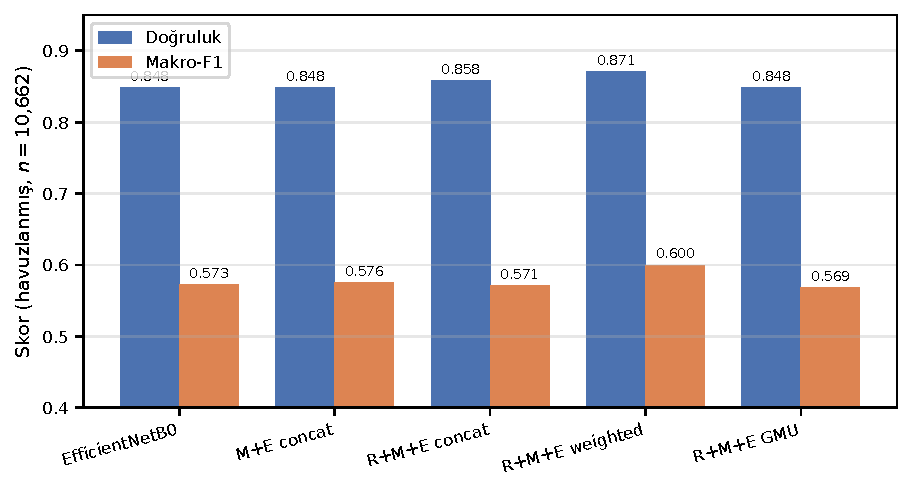
\includegraphics[width=\linewidth]{comparison_bar_chart.pdf}
\caption{Seçilmiş beş 5-katlı yapılandırma için havuzlanmış ($n{=}10{.}662$)
doğruluk ve makro-F1 karşılaştırması.}
\label{fig:bar}
\end{figure}

\begin{figure}[H]
\centering
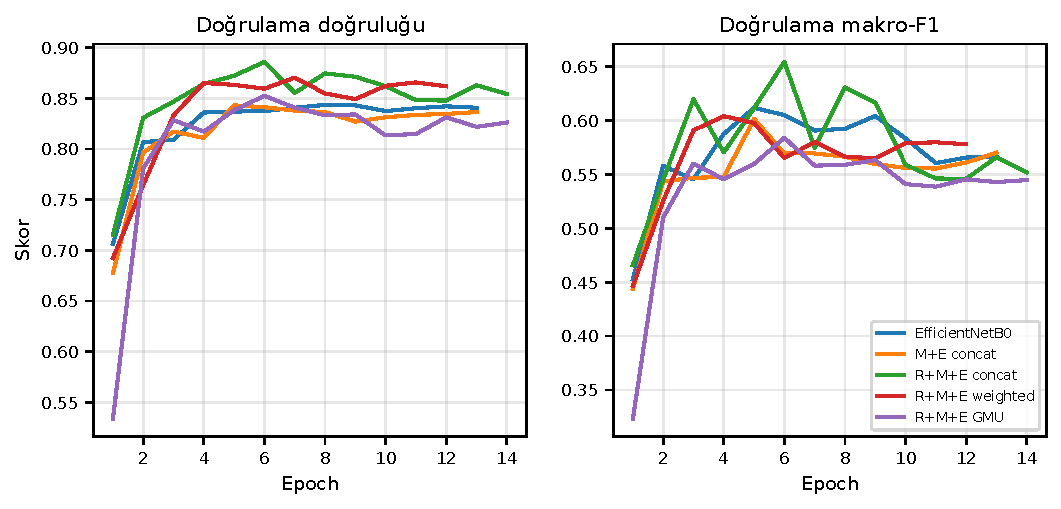
\includegraphics[width=\linewidth]{training_curves.pdf}
\caption{Doğrulama doğruluğu ve makro-F1'in epoch boyunca değişimi (seçilmiş beş
5-katlı yapılandırma, fold 0).}
\label{fig:curves}
\end{figure}

\begin{figure}[H]
\centering
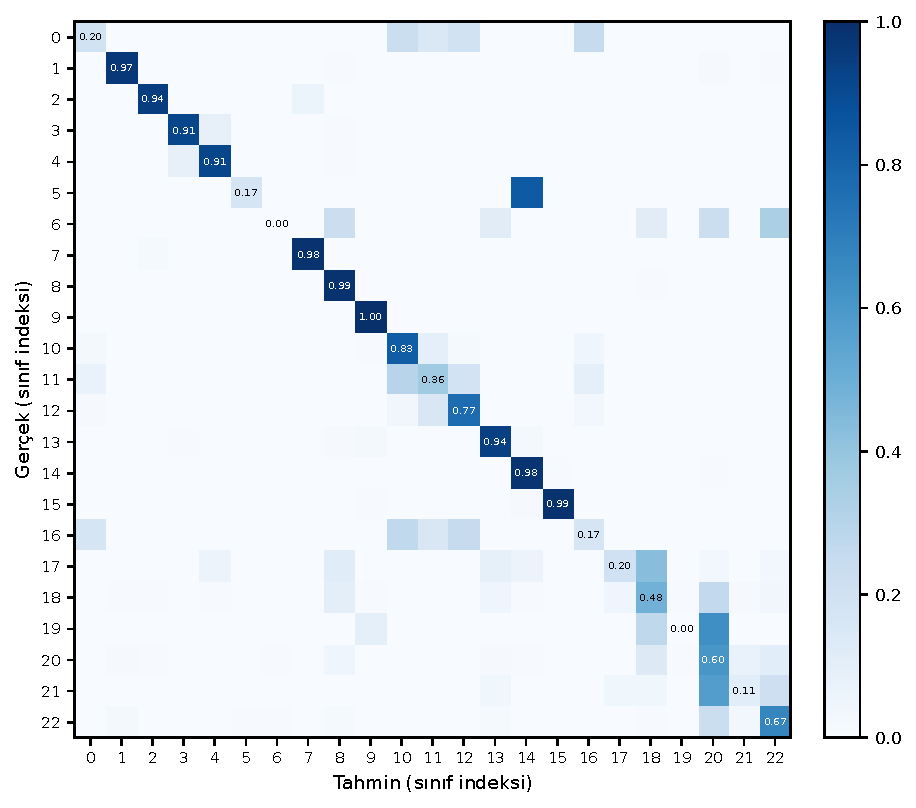
\includegraphics[width=0.8\linewidth]{confusion_matrix_frozen_tta.pdf}
\caption{Nihai model (exp 11 + TTA) için $23\times23$ satır-normalize hata
matrisi, havuzlanmış 5-katlı test ($n{=}10{.}662$). Eksenler sınıf indeksleridir:
{\footnotesize 0=barretts, 1=bbps-0-1, 2=bbps-2-3, 3=dyed-lifted-polyps,
4=dyed-resection-margins, 5=hemorroids, 6=ileum, 7=impacted-stool, 8=normal-cecum,
9=normal-pylorus, 10=normal-z-line, 11=oesophagitis-a, 12=oesophagitis-b-d,
13=polyp, 14=retroflex-rectum, 15=retroflex-stomach, 16=short-segment-barretts,
17=ulcerative-colitis-grade-0-1, 18=ulcerative-colitis-grade-1,
19=ulcerative-colitis-grade-1-2, 20=ulcerative-colitis-grade-2,
21=ulcerative-colitis-grade-2-3, 22=ulcerative-colitis-grade-3.}}
\label{fig:cm}
\end{figure}

\begin{figure}[H]
\centering
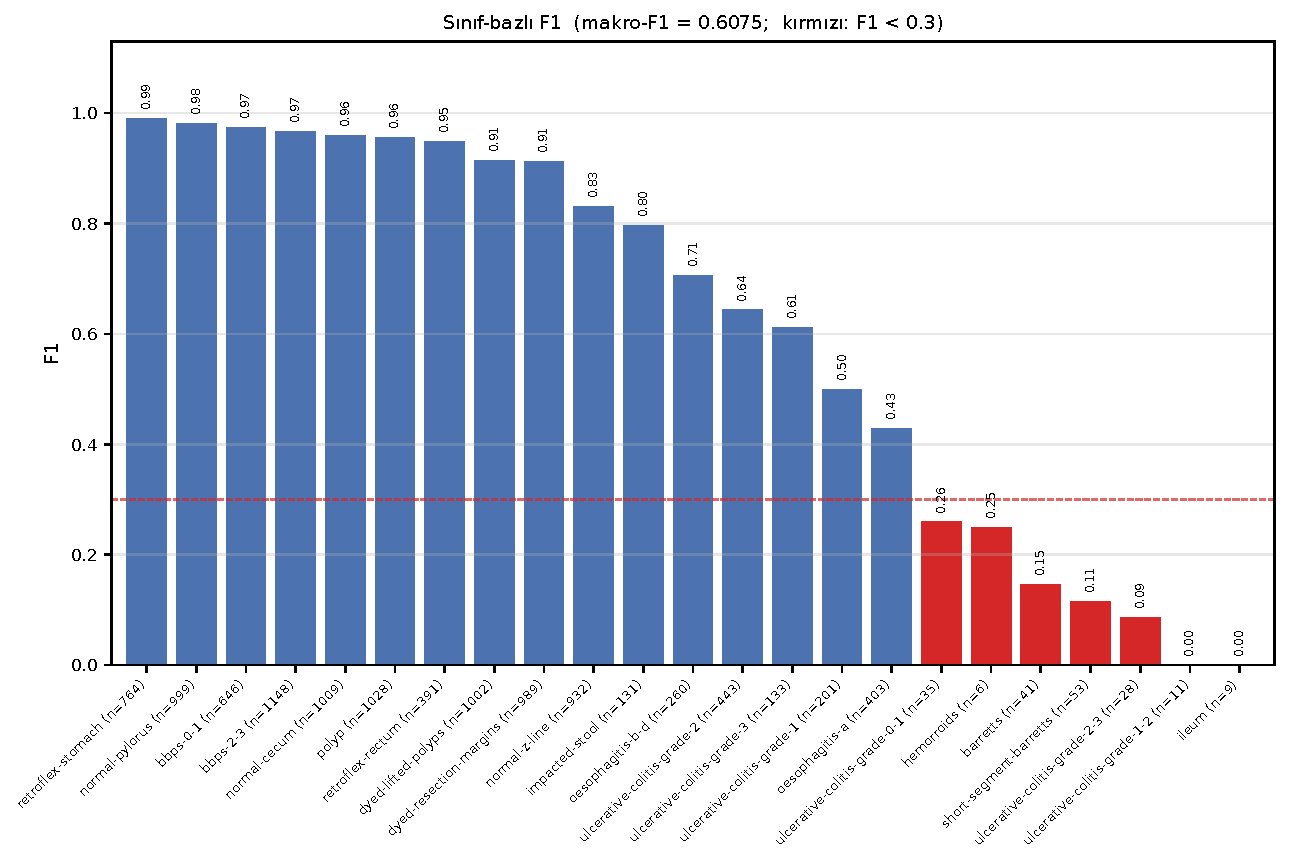
\includegraphics[width=\linewidth]{per_class_f1_frozen_tta.pdf}
\caption{Nihai model için sınıf-bazlı F1 (azalan sırada; kırmızı sütunlar:
F1 < 0.3; kırmızı kesikli çizgi: F1 = 0.3 eşiği). Nadir sınıflardaki çöküş açıkça
görülür.}
\label{fig:perclassf1}
\end{figure}

\subsection{Literatür ile Karşılaştırma}
\label{subsec:contextual}
Karşılaştırmayı iki düzeyde sunuyoruz: (i) bizimle \emph{aynı resmi-bölme
protokolünü} kullanan ve dolayısıyla yakın-doğrudan kıyaslanabilen Borgli ve
ark.\ baseline'ları; (ii) farklı protokol kullanan ve yalnızca \emph{bağlamsal}
olarak anılabilen diğer çalışmalar. Hiçbir durumda doğrudan üstünlük ya da
güncel-en-iyi (SOTA) iddiasında bulunulmamaktadır.

\paragraph{Aynı protokol (resmi bölme).}
Tablo~\ref{tab:cmp-borgli}, aynı resmi-bölme ailesinde raporlanan Borgli ve
ark.~\cite{borgli2020hyperkvasir} baseline'larıyla nihai modelimizi
karşılaştırır. Çok daha \emph{hafif} üçlü füzyonumuz (ResNet50+MobileNetV2+
EfficientNetB0, $\approx$14M omurga parametresi), Borgli'nin \emph{ağır}
ResNet-152+DenseNet-161+MLP füzyonuyla makro-F1'de \textbf{başa baştır}
($0{,}6075$ vs $0{,}605$) ve en iyi tekil omurgaları DenseNet-161'e ($0{,}619$)
yaklaşır; ancak genel doğruluk/mikro-F1 ($0{,}877$ vs $\approx 0{,}907$) ve MCC
($0{,}866$ vs $\approx 0{,}90$) açısından yaklaşık 3--4 puan geridedir. Yani
dengesizliğe duyarlı makro-F1'de ağır modellerle eşitleniyoruz; genel doğrulukta
ise --- daha düşük omurga kapasitesiyle tutarlı biçimde --- onların altında
kalıyoruz. (Borgli iki resmi split ortalaması verir, biz resmi 5-kat kullanırız;
ikisi de resmi-bölme tabanlı, küçük bir fark.)

\begin{table}[H]
\centering
\caption{Aynı resmi-bölme protokolünde karşılaştırma. Borgli değerleri
\cite{borgli2020hyperkvasir} Tablo 3 (iki split ortalaması); bizim değerlerimiz
resmi 5-kat havuzlanmıştır ($n=10{.}662$).}
\label{tab:cmp-borgli}
\begin{tabular}{ll ccc}
\toprule
Yöntem & Omurga(lar) & Makro-F1 & micro-F1/Acc & MCC \\
\midrule
Borgli & ResNet-50 & 0.530 & 0.839 & 0.826 \\
Borgli & ResNet-152 & 0.606 & 0.906 & 0.898 \\
Borgli & DenseNet-161 & 0.619 & 0.907 & 0.899 \\
Borgli & RN152+DN161+MLP & 0.605 & 0.909 & 0.902 \\
\textbf{Bizim} & \textbf{R+M+E + TTA} & \textbf{0.6075} & 0.8765 & 0.8662 \\
\bottomrule
\end{tabular}
\end{table}

\paragraph{Bağlamsal (farklı protokol --- baş-başa değil).}
Tablo~\ref{tab:cmp-context} farklı bölme/ön işleme kullanan çalışmaları listeler;
protokol farkı nedeniyle baş-başa kıyaslanamazlar. Effimix~\cite{ramamurthy2022effimix}
$\approx \%98$ doğruluk ($0{,}97$ makro-F1) bildirir; ancak bu sonuç veriyi
$\sim$23.000'e augment edip sınıfları dengeleyen ve resmi-olmayan bir bölme
kullanan bir kuruluma dayanır (iyimser yanlılık). GastroViT~\cite{gastrovit2025}
23-sınıf için $0{,}92$ doğruluk / $0{,}64$ makro-F1 (tek split) verir; 16-sınıflı
sonuçları farklı bir görev olduğundan bizim 23-sınıflı sonuçlarımızla
\emph{karıştırılmaz}. Dürüst, resmi-protokol bandında 23-sınıf makro-F1
$\approx 0{,}53$--$0{,}62$ aralığındadır ve bizim $0{,}61$ değerimiz bu banttadır.

\begin{table}[H]
\centering
\caption{Bağlamsal karşılaştırma (farklı protokol --- baş-başa DEĞİL).
``Effimix T5'' = ilgili değerler Effimix'in karşılaştırma tablosundan (Tablo 5)
aktarılmıştır.}
\label{tab:cmp-context}
\begin{tabular}{lll cc}
\toprule
Çalışma & Yöntem & Protokol & Makro-F1 & Acc \\
\midrule
Effimix~\cite{ramamurthy2022effimix} & EffNetB0+Effimix & augment+dengeleme, resmi-olmayan & 0.97 & 0.98 \\
GastroViT~\cite{gastrovit2025} & MobileViT topluluğu & 64:16:20 tek split & 0.64 & 0.92 \\
He ve ark.\ (Effimix T5) & ResNet-152+MobileNetV3 & belirsiz & 0.66 & -- \\
Galdran (CNN--BiT, Effimix T5) & BiT & belirsiz & 0.92 & -- \\
Galdran (MNV2+ResNeXt, Effimix T5) & MNV2+ResNeXt & belirsiz & 0.64 & 0.65 \\
\bottomrule
\end{tabular}
\end{table}

\paragraph{AUC nüansı.}
Eşik-bağımsız makro tek-vs-rest ROC-AUC değerimiz ($0{,}967$), Effimix'in
bildirdiği AUC'ye ($0{,}977$) yakındır; oysa makro-F1'imiz ($0{,}61$) onunkinin
($0{,}97$) çok altındadır. Bu, büyük F1 farkının sıralama kalitesinden değil,
çalışma noktası / sınıf dengesi / protokol farkından kaynaklandığını gösterir
(bu AUC kıyası da çapraz-protokoldür ve yalnızca açıklayıcıdır).

% =====================================================================
% 5. TARTIŞMA (Discussion) — EN KRİTİK BÖLÜM (%25)
% Evidence base: docs/results_progress.md (key findings), docs/experiment_log.md,
%                docs/report/AGENT_REPORT_RULES.md §4-§7.
% Address the assignment §5.5 questions explicitly. Report neutral/negative
% results honestly. No SOTA, no protocol-mismatched head-to-head claims.
% =====================================================================
\section{Tartışma}
\label{sec:discussion}

% TODO: Hangi omurga ağ daha iyi özellik öğrendi ve neden?
%       Frozen'da EfficientNetB0 en iyi tekil (F1 0.5586); CV'de weighted füzyon kazandı.
\TODO{Hangi CNN daha iyi özellik öğrendi? (frozen E en iyi tekil; gerekçe).}

% TODO: Füzyon performansı artırdı mı? Concat vs weighted CI ayrımı
%       (exp 11 lower 0.5814 > exp 10 upper 0.5799). GMU concat'i geçemedi (Δ≈0.002).
\TODO{Füzyon yardımcı oldu mu? concat vs weighted CI ayrımı; GMU nötr sonucu.}

% TODO: En iyi kombinasyon — üçlü weighted fine-tune (exp 11), CV F1 0.5892,
%       pooled 0.6000. Fold-0 sıralamasının yanıltıcı olduğu (concat>weighted) ve
%       5-fold ile tersine döndüğü açıklanacak (metodolojik ders).
\TODO{En iyi kombinasyon (exp 11) ve fold-0 yanılgısının açıklaması.}

% TODO: Güçlü/zayıf yönler — nadir sınıflar (support ≤ 10) F1=0; hata matrisi
%       rastgele değil, anlamsal/görsel olarak yakın çoğunluk sınıfına soğuruluyor.
\TODO{Güçlü/zayıf yönler; nadir-sınıf çöküşü (support ≤ 10) ve hata yapısı.}

% TODO: Sınıf dengesizliği etkisi — accuracy 0.87 vs macro-F1 0.60 farkı;
%       weighted-F1 0.87 / MCC 0.86. macro-F1'in neden headline olduğu.
\TODO{Dengesizlik etkisi; accuracy$\leftrightarrow$macro-F1 farkı; macro-F1 gerekçesi.}

% TODO: Hangi transfer learning yaklaşımı daha başarılı ve NE KADAR SÜRDÜ?
%       Fine-tune CV ortalamasında frozen'ı geçti. Süre: Tablo 4'e bağlı (HENÜZ YOK).
\TODO{Frozen vs fine-tune sonucu + süre yorumu (Tablo 4 üretilince bağlanacak).}

% TODO: Literatür ile dürüst konumlandırma — bizim ~0.60 macro-F1, Borgli'nin
%       resmi-split ~0.62 bandında; Effimix 0.97 farklı protokol (augment+balance+
%       non-official split) → doğrudan kıyaslanamaz. Saklama, açıkla (§8 dürüstlük).
\TODO{Dürüst literatür konumlandırması (protokol farkı; SOTA iddiası YOK).}

% NOTE: En önemli sonuçların yorumu ve sınırlamalar öğrenci tarafından elle
%       gözden geçirilecek (AGENT_REPORT_RULES.md §9).

% =====================================================================
% 6. SONUÇ (Conclusion)
% Summarize actual findings only. Introduce NO new results.
% Evidence base: docs/FINAL_MODEL.md, docs/results_progress.md, docs/decisions.md.
% =====================================================================
\section{Sonuç}
\label{sec:conclusion}

Bu çalışmada, HiperKvasir 23-sınıf gastrointestinal endoskopi görevi için üç
önceden eğitilmiş CNN omurga ağının (ResNet50, MobileNetV2, EfficientNetB0)
özelliklerini birleştiren, MLP sınıflandırıcılı bir füzyon mimarisi, resmi
5-katlı protokol altında kontrollü biçimde değerlendirilmiştir. Karşılaştırmalar
omurga ağ, füzyon (birleştirme / ağırlıklı / GMU) ve transfer öğrenme (frozen /
fine-tune) eksenlerinde yürütülmüş; ana ölçüt olarak makro-F1 kullanılmıştır.
Resmi 5-katlı protokolde en iyi yapılandırma üçlü ağırlıklı fine-tune (exp 11)
olmuş; nihai model bu yapılandırmanın TTA'lı sürümüdür (havuzlanmış
makro-F1 $0{,}6075$). Sayısal sonuçlar ve yorumlar
Bölüm~\ref{sec:results}--\ref{sec:discussion}'de verilmiştir.

\paragraph{Sınırlamalar.}
En iyi yapılandırmanın üzerinde değerlendirilen toplamsal ablasyonların --- focal
loss, TTA ve sızıntısız seed topluluğu --- hiçbiri \%95 güven aralığı düzeyinde
en iyi çapraz-entropi yapılandırmasını istatistiksel olarak geçememiştir; bu, bu
ek tekniklerle elde edilebilecek iyileşmenin sınırlı kaldığını gösterir. Kalan açığın başlıca kaynağı, çok düşük destekli
(support $\le 10$) nadir sınıflardır; bu, kayıp/çıkarım/topluluk düzeyindeki
ayarlamalarla kapanmayan bir veri kıtlığı sınırıdır. Ayrıca, farklı protokol ve
ön işleme kullanan literatür sonuçlarıyla doğrudan baş-başa karşılaştırma
yapılamaz; yalnızca resmi-bölme tabanlı sonuçlar bağlamsal bir çapa sağlar. Son
olarak, final model tek tohumla (seed 42) eğitilmiştir.

\paragraph{Gelecek çalışma.}
İleride, nihai model üzerinde yorumlanabilirlik analizleri --- Grad-CAM++
\cite{chattopadhyay2018gradcampp} ile sınıf-etkin bölge görselleştirmesi ve
birleşik 512-boyutlu özelliklerin UMAP~\cite{mcinnes2018umap} ile izdüşürülmesi
--- eklenebilir. Eğitim reçetesinin daha ileri bir sürümü (recipe-v2) ve daha
geniş bir tohum topluluğu da, özellikle nadir sınıflar için, olası iyileştirme
yönleri olarak değerlendirilebilir. Bu yönler bu raporun kapsamı dışındadır ve
gelecek çalışma olarak bırakılmıştır.


% ---------------------------------------------------------------------
\bibliographystyle{plain}
\bibliography{references}

\end{document}
